\section{Motivation}
{Die Ausgaben für das Internet der Dinge (IoT) wird weltweit, laut Statista, bis zum Jahr 2022 auf 1000 Milliarden US-Dollar steigen. Im Vergleich zum Jahr 2019 bedeutet dies, eine Steigerung von über 40\%.}\cite{STATISTA01:IOT} Bei einem solch starken Trend in der Informatik-Branche sollten sowohl Studenten, als auch Professoren dessen Grundlagen kennen.
Deshalb ist im Rahmen des Faches Softwarearchitektur an der technischen Hochschule Rosenheim diese Ausarbeitung geschrieben worden. Das Ziel ist es openHAB, ein Heimautomatisierungs-Tool, aus praktischer und technischer Sicht zu untersuchen. Außerdem wird dabei auf die Aspekte Markttauglichkeit und Benutzbarkeit in der Praxis eingegangen.

\section{Was ist openHAB?}
\label{s:what-is-openHAB}
openHAB ist eine technologie unabhängige Open-Source-Automatisierungs-Software für das Smart-Home.
Das Projekt wurde von Kai Kreuzer 2010 erstmals initiiert und wird mittlerweile durch die Community weiterentwickelt. Die Software ist hauptsächlich in Java und der Auszeichnungssprache XML geschrieben. Seit dem 16. Dezember 2019 ist die Version 2.5 erhältlich.\\
\\
Auf der offiziellen Website von openHAB \url{https://www.openHAB.org/} sind drei klare Hauptziele definiert, die diese Software erreichen soll. Dabei ist ein Ziel die Plattformunabhängigkeit. Somit kann openHAB sowohl auf Linux, MacOS oder Windows betrieben werden. Auch das Hosten mit Docker oder einem Raspberry Pi wird unterstützt.\\
Weiterhin soll es durch die Plugin-Architektur möglich sein, fast jedes Gerät zu integrieren.
Es werden über 200 Technologien und mehrere tausende verschiedene Geräte unterstützt.\\
Das dritte Ziel weißt auf die vielen verschiedenen Automatisierungsmöglichkeiten hin, die openHAB zu bieten hat. Dabei werden Auslöser (in Englisch: Trigger), Aktionen, Skripte und auch Voice-Kontrolle genannt.

\section{Bewertung von openHAB}
In diesem Kapitel wird das Open-Source Projekt openHAB untersucht und bewertet. Es befindet sich auf Github unter \url{https://github.com/openHAB/openHAB-core}. Die hierfür verwendeten Kriterien sind orientiert an der \textit{QAware Open Source Quick-Check Liste}.
Diese beinhaltet:
\begin{longtable}{| p{3cm} | p{12cm}|}
	\hline
	\textbf{Kriterium} & \textbf{Beschreibung} \\
	\hline \hline
	\centering Projekt Aktivität & Gibt es?
	\begin{itemize}
		\item Mindestens 1 Release im letzten Jahr
		\item Mindestens 3 aktive Contributer
		\item Stetige Commit-Aktivität von mindestens 1x pro Monat
	\end{itemize}\\
	\hline
	\centering Reifegrad & Existiert eine stabile Version > 1.0?  \\
	\hline
	\centering Lizenz & Für welche Zwecke kann das Projekt genutzt werden? \\
	\hline
	\centering Support & Existiert Issue-Tracking und eine Antwortzeit auf Tickets unter 24h? \\
	\hline
	\centering Dokumentation & Existiert?
	\begin{itemize}
		\item Api-Dokumentation
		\item Getting Started Tutorial
		\item Aktuelle Dokumentation
	\end{itemize} \\
	\hline
	\caption{openHAB Projektbewertungskriterien}
	\label{table:openHAB-judgement-criteria}
\end{longtable}

Der Online-Dienst \textbf{Open Hub}, ehemals \textbf{Ohloh} genannt, katalogisiert Open-Source Software-Projekte. Für jedes Projekt werden Daten wie Name, Beschreibung und Quellcode erfasst. Basierend auf diesen Daten erstellt Open Hub eine Statistik, die es ermöglicht Codeanalyse, Projektmitarbeiter, Aktivitäten und eine Übersicht zu erhalten. Dabei fließen auch Daten weiterer Open-Source Projekte ein, um aussagekräftige Statistiken zu erhalten und Aussagen treffen zu können.\\
\\
{In der Auswertung über openHAB ist zu finden, dass 2019 über 380 Entwickler aktiv an dem Projekt mitgearbeitet haben. Somit ist openHAB unter den top 2\% der größten Projektteams auf Open Hub.\\
Des Weiteren ist ein stetiger Anstieg von Interesse erkennbar. Dies wird durch den Vergleich von Codebeiträgen des aktuellen Jahrs und des Vorjahres begründet.\\
Insgesamt haben über 1140 Entwickler bereits mehr als 20000 Beiträgen in Form von Programmcode zum Projekt beigetragen. Der Umfang des zu 98\% in Java geschriebenen Codes beträgt mehr als 1.5 Millionen Zeilen. Davon wurden circa 31\% dokumentiert. Dies entspricht dem durchschnittlichen Wert aller Java Open-Source Projekte, welche auf Open Hub registriert sind.}\cite{OPENHUB01:OH} Die hierbei angegeben Werte beziehen sich auf alle Projekte und Subprojekte von openHAB. Eine Übersicht hierfür ist unter \url{https://github.com/openHAB} zu finden.\\
\\
Wie bereits im Kapitel \ref{s:what-is-openHAB} erwähnt, ist openHAB aktuell in der Version 2.5 erhältlich. Daraus lässt sich auf einen stabilen Codestand schließen.\\
Des Weiteren ist das Projekt unter einer EPL-2.0 Lizenz veröffentlicht. Dies erlaubt sowohl die private als auch kommerzielle Nutzung. Hinzu kommt die Möglichkeit für Modifizierung und Weiterverbreitung.\cite{LICENSE01:EC}
\\
\\
Des Weiteren wird die Qualität des Supports evaluiert. Hierfür stellt Github einen Issue-Tracker zur Verfügung. Beim Teilprojekt openHAB-core wurden über 1250 Issues verfasst, wovon bei circa 90\% bereits die Bearbeitung abgeschlossen ist.\cite{GITHUB01:OS} Dies lässt auf eine aktive Nutzung des Issue-Trackers schließen und bietet somit eine hilfreiche Support-Möglichkeit. Hierfür ist vor allem das Label \textbf{Bug} von Bedeutung. Eine Stichprobenartige Untersuchung von Issues dieses Types hat eine durchschnittliche Antwortzeit in unter 24h ergeben. Dies wurde anhand des ersten Kommentars gemessen. Zudem wurden bereits circa 83\% der insgesamt 68 dokumentierten Bugs gelöst.
\\
\\
Abschließend wird der Zustand der Dokumentation untersucht.
Das Getting-Started Tutorial ist ausführlich und aktuell. Die darüber hinausgehende Basisdokumentation ist vollständig. Nur in Spezialfällen, wie beispielsweise der Implementierung von Services, ist die Dokumentation lückenhaft.\cite{openHAB01:OH}

\subsection{Fazit der Bewertung}
\begin{longtable}{| p{3cm} | p{10cm}| c |}
	\hline
	\textbf{Kriterium} & \textbf{Beschreibung} & \textbf{Erfüllt?} \\
	\hline \hline
	\centering Projekt Aktivität & Gibt es?
	\begin{itemize}
		\item Mindestens 1 Release im letzten Jahr
		\item Mindestens 3 aktive Contributer
		\item Stetige Commit-Aktivität von mindestens 1x pro Monat
	\end{itemize} & \checkmark \\
	\hline
	\centering Reifegrad & Existiert eine stabile Version > 1.0? & \checkmark \\
	\hline
	\centering Lizenz & Für welche Zwecke kann das Projekt genutzt werden? & \checkmark \\
	\hline
	\centering Support & Existiert Issue-Tracking und eine Antwortzeit auf Tickets unter 24h? & \checkmark \\
	\hline
	\centering Dokumentation & Existiert?
	\begin{itemize}
		\item Api-Dokumentation
		\item Getting Started Tutorial
		\item Aktuelle Dokumentation
	\end{itemize} & X/\checkmark \\
	\hline
	\caption{openHAB Projektbewertungskriterien Ergebnis}
	\label{table:openHAB-judgement-criteria-result}
\end{longtable}

\subsection{Weiterführende Bewertungen}
openHAB wurde bereits in der Bachelorarbeit von Pirmin Gersbacher vom Jahr 2017/2018 anhand von Usecases untersucht und verglichen. Dabei kam er zu folgender Ergebnis.

\begin{minipage}{\textwidth}
	\centering
	\captionsetup{type=figure}
	\includegraphics[width=0.8\textwidth]{\figdir/comparison-openHAB.PNG}
	\caption{Vergleich openHAB und anderen Heimautomatisierungstools von 2017/2018 \label{fig:comparison-openHAB}}
\end{minipage}
\smallskip
 
In Tabelle \ref{fig:comparison-openHAB} sind die unterschiedlichen Gebiete der Untersuchung auf der linken Seite zu finden. In der horizontalen sind die einzelnen Heimautomatisierungs-Tools aufgelistet. In der jeweiligen Zelle, basierend auf Reihe und Spalte, sind die Bewertungen festgehalten. Dabei zeigt ein blau markiertes Feld, welches das beste Tool für ein Gebiet ist.\\
openHAB sticht dabei nicht sonderlich heraus. Allerdings ist es in keinem der aufgelisteten Kategorien negativ bewertet.\\
Der Autor schreibt in seiner Bachelorarbeit, dass er persönlich auf openHAB setzen würde. Dies liegt einerseits daran, dass die Entwickler von openHAB stark an Vereinfachung von komplizierteren Komponenten arbeitet. Andererseits sollen aber auch komplexere Automationen, durch die Nähe von Framework und Java, möglich sein.\cite{BA01:OPH}
\\
\\
Dadurch, dass die Bachelorarbeit von P. Gersbacher 2017/2018 veröffentlicht wurde, stellt diese nicht mehr den aktuellen Stand dar. Seitdem wurde die neuere Version 2.5 entwickelt. Diese beinhaltet einige fundamentale Veränderungen. Dabei sind Anpassungen, um eine verbesserte Nutzung einhergegangen. Auf diese Weise können sowohl openHAB-Entwickler, als auch Entwickler, die openHAB als Basis verwenden, deutlich einfacher programmieren, laut Kai Kreuzer in dessen Online Blog Post über das openHAB 2.5 Release.\cite{openHAB02:OH}\\
In dieser Arbeit wird auf die speziellen Änderungen der Version 2.5 eingegangen. Dabei werden die Ergebnisse von P. Gersbacher als zusätzliche Quelle genutzt.


\section{Komponenten von openHAB}\label{sec:technischeSicht}
In diesem Kapitel werden die grundlegenden Komponenten dargestellt, welche openHAB verwendet. Des Weiteren wird auf die  Beziehung der Komponenten untereinander eingegangen.
Ein Kernaspekt welcher in diesem Kapitel zum Vorschein kommt ist, dass es in der Regel den "'einen Weg"'nicht gibt. openHAB bietet meist mehrere Wege ein Ziel zu erreichen, je nach Vorlieben des Nutzers. So ist es zum Beispiel möglich ein Gerät über die Web-Oberfläche als auch über geschriebenen Code zu integrieren. Das gleiche ist auch bei Rules zu sehen, welche entweder über ein Add-On in der Web-Oberfläche definiert werden können oder über Code. Dieses Konzept ist ein Grundgedanke, der von openHAB verfolgt wird, welcher allerdings zu Verwirrung führen kann, da bei anfänglichen Umgang mit openHAB nicht unbedingt klar ist, wie ein gewünschtes Ziel erreicht werde kann.
In Tabelle \ref{table:openhub-components} sind einige der Grundlegenden Komponenten aus openHAB zur schnellen Übersicht aufgeführt. Detailliert werden diese in den entsprechenden Unterkapiteln beschrieben.

\begin{longtable}{| p{4cm} | p{11cm}|}
	\hline
	\textbf{Komponente} & \textbf{Beschreibung} \\
	\hline \hline
	\centering Add-Ons & Erweiterungen, welche die Funktionalitäten von openHAB erhöhen. \\
	\hline
	\centering Bindings & openHAB-Komponenten, welche die Schnittstelle zu fremd Systemen darstellt.  \\
	\hline
	\centering Things & Repräsentation von physischen Geräten/Services in openHAB. \\
	\hline
	\centering Items & Darstellung von Eigenschaften und Ressourcen von openHAB - Thing bezogen \\
	\hline
	\centering Channels & Übertragungskanal zwischen "`Items"' und "`Things"'. \\
	\hline
	\centering Rules & Automatisierungsregeln, in Wenn-Dann-Struktur.\\
	\hline
	\centering Sitemaps & Individuelle Benutzeroberfläche, welche Informationen präsentiert und Interaktionen ermöglicht.\\
	\hline
	\caption{openHAB Komponenten}
	\label{table:openhub-components}
\end{longtable}

\subsection{Add-Ons}\label{sec:add-ons}
openHAB verwendet das Konzept von Add-Ons als Teil ihrer zusammensteckbaren Architektur (pluggable architecture). Dadurch, dass vordefinierte Bereiche von openHAB erweitert werden können, wird openHAB der Anforderung gerecht "'alles"' zu Integrieren. Das Konzept der Add-Ons ermöglicht es außerdem nur benötigte Module zu installieren bzw. zu verwenden wodurch openHAB schlank, leicht und überschaubar bleibt. Die Bereiche in denen openHAB offen ist, um erweitert zu werden sind nach \cite{openHAB04:OH}:
\begin{itemize}
	\item Bindings
	\item Automation-Engine-Modules
	\item Transformations / Profiles
	\item IO-Services
	\item Persistence-Services
	\item Audio \& Voice
\end{itemize}
Um den Rahmen dieser Arbeit nicht zu übersteigen wird nur auf Bindings detaillierter eingegangen, siehe Kapitel \ref{sec:Bindings}. Bei den nicht näher beschriebenen Add-Ons handelt es bei Automation-Engine-Modules um Bedingungen oder Aktionen, welche für Rules oder Scripte verwendet werden können. Transformations / Profiles können genutzt werden um Werte welche durch Channels übertragen werden zu tranformieren / modfizieren. IO-Services ermöglichen es interne Schnittstellen von openHAB nach außen aufzumachen. Dies geschieht z.B. bei der REST-Api, dem HomeKit für Apple oder dem Hue Emulation Service für Philips. Persistence-Services können genutzt werden um den Status von Items z.B. in Datenbanken abzuspeichern und wieder abzurufen. Und bei Audio \& Voice handelt es sich um Services, welche genutzt werden, um Audioquellen abzuspielen oder Stimminteraktionen mit Nutzern zu ermöglichen.

\subsection{Bindings} \label{sec:Bindings}
Bindings sind Komponenten, welche es ermöglicht Systeme oder Geräte mit openHAB zu integrieren. Mit einem Binding kann sowohl ein physisches Geräte wie z.B. ein LG Fernseher mit WebOS als auch eine Service z.B. Spotify angebunden werden. Die Bindings sind dabei meist soweit abstrahiert, dass nicht jedes einzelne Model bzw. Version ein eigenes Binding benötigt.
Nach der Installation eines Bindings, was über die Web-Oberfläche oder per Code geschehen kann, ist openHAB in der Lage Geräte/Systeme im Netzwerk zu finden. Mittels Bindings können auch Geräte/Systeme integriert werden, welche wiederum die Steuerung für andere Geräte übernehmen, z.B. Hue-Bridge oder Bluetooth. Diese Geräte/Systeme wiederum ermöglichen es i.d.R. nach dem Hinzufügen in openHAB, dass durch das Binding Kindkomponenten gefunden und ebenfalls zu openHAB hinzugefügt werden können. Dadurch ist es möglich, wie im Falle des Hue-Systems nicht nur die Hue-Bridge, sondern alle mit der Hue-Bridge verbundenen Lampen einzeln in openHAB zu integrieren und dadurch zu steuern. Dieses Ansteuern von einzelnen Kindkomponenten im Falle des Hue-Systems, wäre durch ZigBee theoretisch möglich, würde aber einen sehr hohen und unnötigen Aufwand bedeuten.
Laut openHAB gibt es aktuell über 300 Bindings welche es ermöglichen über 2000 Things anzusprechen \cite{OPENHUB00:OH}.

\subsection{Things}
Things stellen die Repräsentation von physischen Geräten/Services innerhalb von openHAB dar. Sie bestehen neben verschiedenen Status und Konfigurationsinformationen aus Channels, welche für die Ansteuerung der Things benötigt werden und näher in Kapitel \ref{sec:channels} beschrieben werden.
Things können auf drei verschiedene Arten zu openHAB hinzugefügt werden. Diese sind:
\begin{itemize}
	\item Per Web-Oberfläche automatisch: Nachdem das für das Thing benötigte Binding installiert wurde, erscheint das Thing in der Inbox, siehe Abbildung \ref{fig:thing-add-paper-ui}. Von dieser Inbox aus, kann das Thing mit wenigen Klicks openHAB hinzugefügt werden. Durch diese Methode werden alle nötigen Einstellungen für das Thing automatisch getroffen. Diese können nachträglich bearbeitet werden z.B. umbenannt werden. 
\end{itemize}
{
	\centering
	\captionsetup{type=figure}
	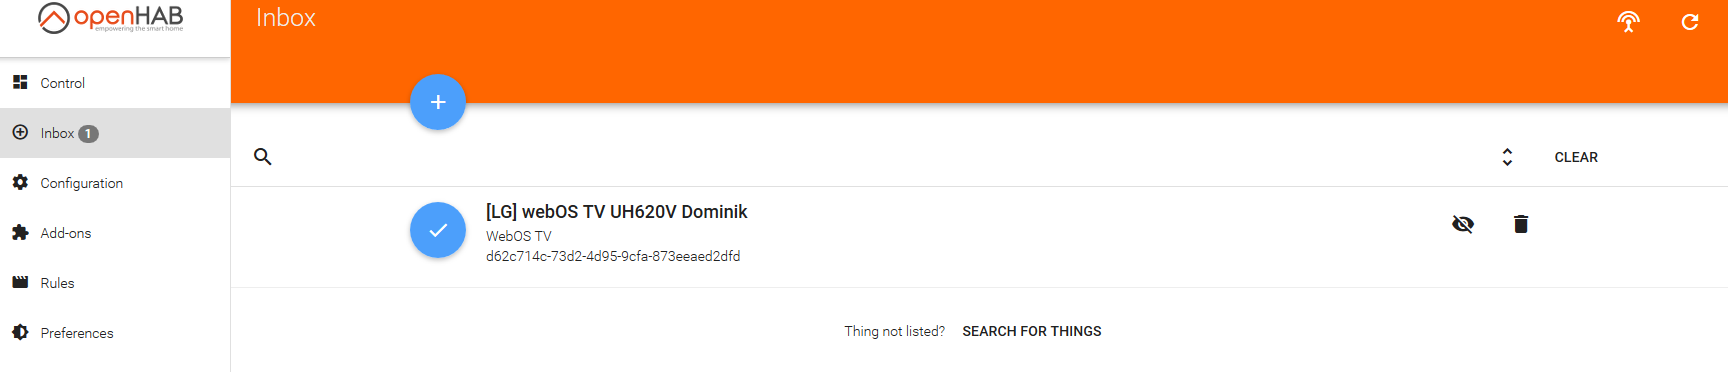
\includegraphics[width=1\textwidth]{\figdir/thing_add.PNG}
	\caption{Thing per Web-Oberfläche \label{fig:thing-add-paper-ui}}
}	
\begin{itemize}	
	\item Per Web-Oberfläche Manuell: Das manuelle Hinzufügen von Things ermöglicht volle Einstellungsfreiheit für Things. Dazu zählen ID, Bezeichnung, IP-Adresse und Konfigurationsparameter. Dies ist in Abbildung \ref{fig:thing-add-paper-ui-manuel} zu sehen. Diese Einstellungsfreiheit setzt allerdings auch voraus, dass der Nutzer weiß, welche Informationen er in welches Feld eintragen will/muss. Genau wie beim automatischen Erkennen können die Einstellungen nachträglich geändert werden. 
\end{itemize}
{
	\centering
	\captionsetup{type=figure}
	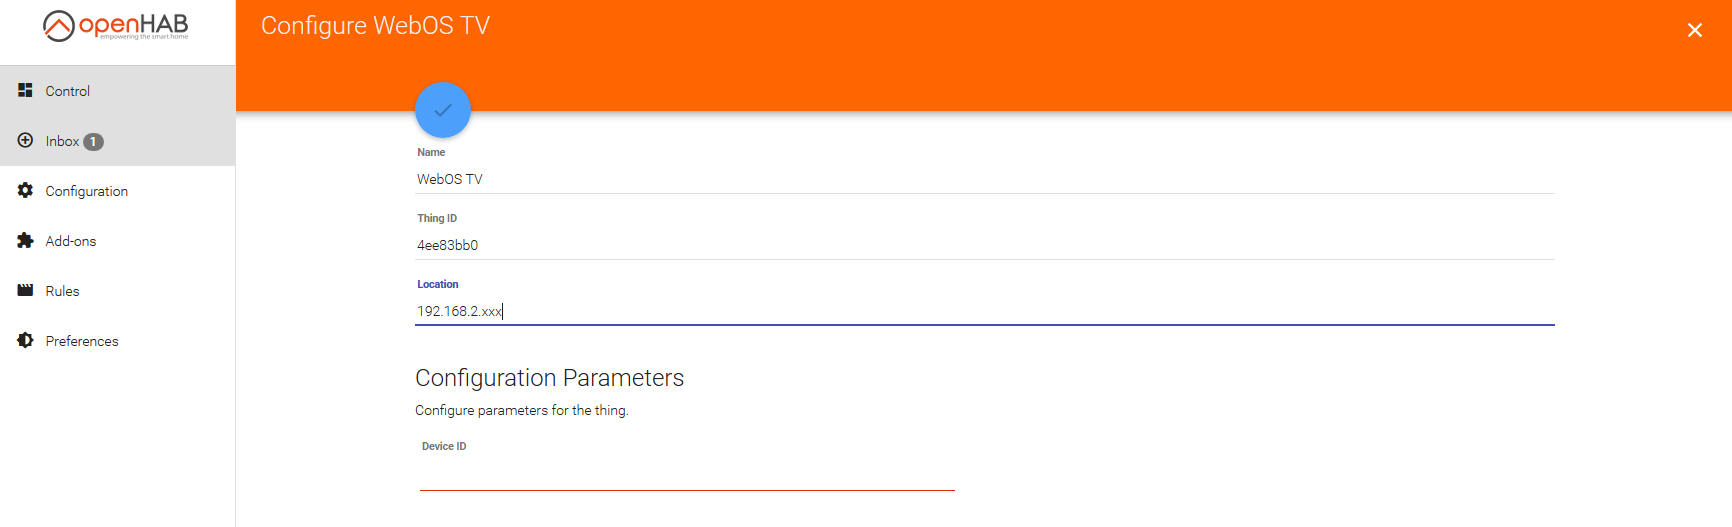
\includegraphics[width=1\textwidth]{\figdir/thing_add_manuel.PNG}
	\caption{Thing per Web-Oberfläche Manuell \label{fig:thing-add-paper-ui-manuel}}
}
\begin{itemize}	
	\item Per Code. Ermöglicht und benötigte komplette manuelle Eingabe aller nötigen Informationen im Dateiordner  \textit{openHAB-config/things/}. Diese sind wie im einfachen Beispiel Abbildung \ref{fig:thing-add-code} Binding-Pfad, IP-Adresse, und ID. Um dies zu vereinfachen sind in der Dokumentation Beispiele für die verschiedenen Bindings mit zugehörigen Things zu finden.
\end{itemize}
{
	\centering
	\captionsetup{type=figure}
	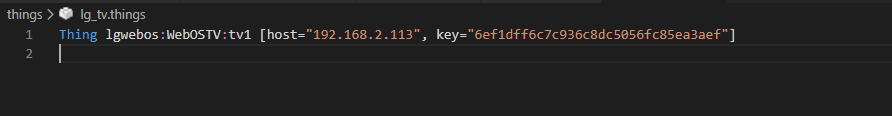
\includegraphics[width=1\textwidth]{\figdir/thing_add_code.PNG}
	\caption{Thing per Code \label{fig:thing-add-code}}
}

\subsection{Channels} \label{sec:channels}
Channels sind Kommunikationswege welche von Things angeboten werden und diese mit Items verbinden. Mit Hilfe der Channels werden Aktionen, welche Things auszuführen haben, Parameter übergeben. So bietet der verwendete LG Fernseher, wie in Abbildung \ref{fig:channel-list} zu sehen, eine Liste von Channels an, welche Daten für Aktionen übertragen um diese Auszuführen. Das heißt, dass Channels sowohl die Kommunikationswege mit zugehörigen Parameter repräsentieren als auch Aktionen, welche Things ausführen können. Eine gewünschte Aktion eines Things kann ohne den passenden Channel diese Aktion nicht ausgeführt werden.

{
	\centering
	\captionsetup{type=figure}
	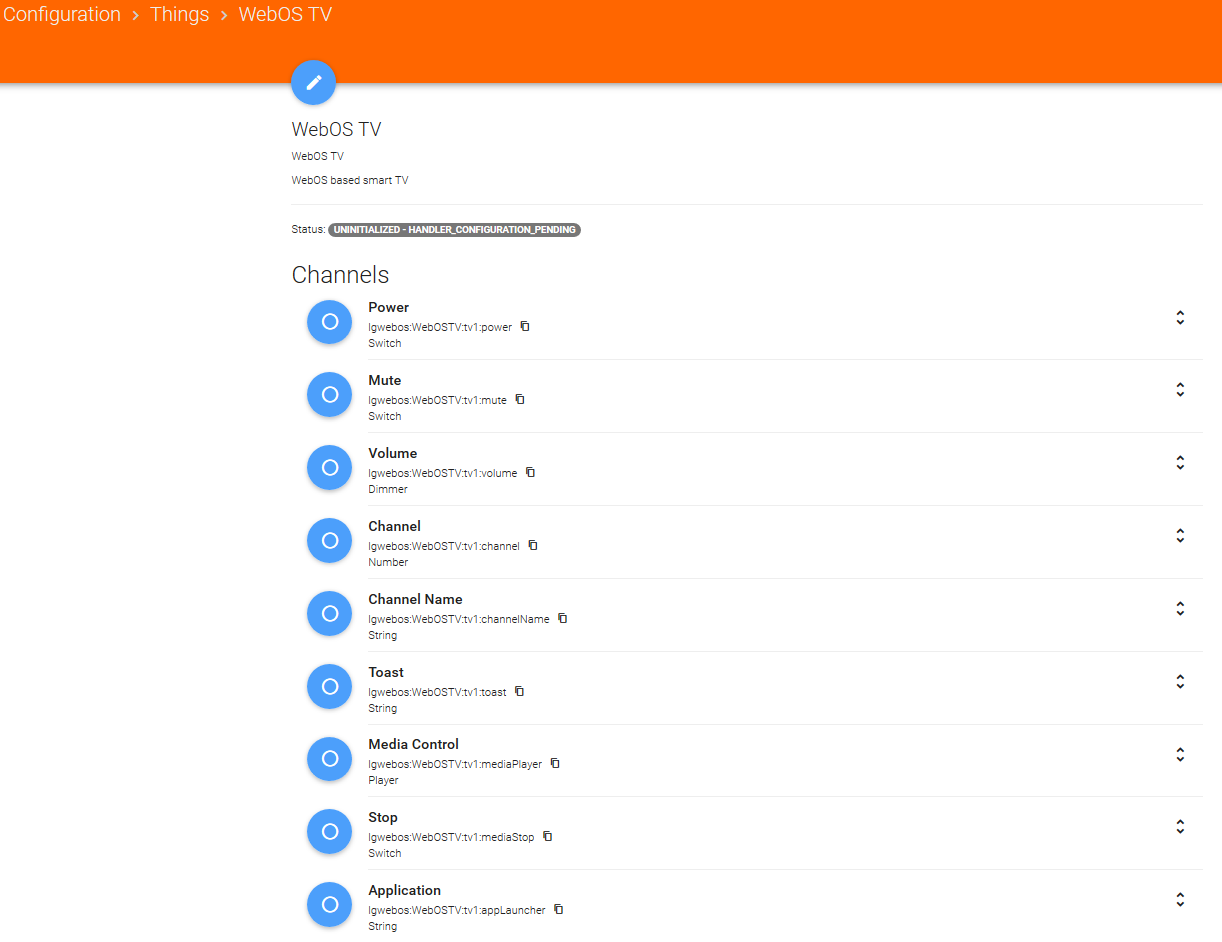
\includegraphics[width=1\textwidth]{\figdir/channel-list.PNG}
	\caption{Channel Liste\label{fig:channel-list}}
}

\subsection{Items}
Der Begriff Item oder zu deutsch Ding, kann missverständlich aufgefasst werden. Bei einem Item handelt es sich um alle Informationen, welche es über eine Aktion gibt. So hat ein Item u.a. Bezeichnung, Kategorie, Typ, Status als auch Konfigurationen z.B. dass nur Werte von 0 - 50 übertragen werden. Diese Informationen werden benötigt, um Gruppierungen zu ermöglichen, den Status eines Gerätes abzufragen (z.B. Lautstärke eines Fernsehers) und auch mit einem Thing zu kommunizieren bzw. Aktionen auszuführen. Der Typ eines Items gibt an, welche Basistypen von dem Item akzeptiert/konsumiert werden können. Solche Basistypen können sowohl einfache, aus der Programmierung, bekannte Typen wie String, Number, DateTime usw. sein, als auch komplexere openHAB spezifische Typen wie Location, Player oder Switch. Eine komplette Auflistung ist unter \url{https://www.openHAB.org/docs/configuration/items.html#type} zu finden.

Items sind essentiell um Aktionen auf der Web-Oberfläche dazustellen. So können diese in Gruppen oder einzeln dargestellt werden um als Statusanzeige und/oder als manuelle Steuerung des Smart Homes zu agieren. Für diese Steuerung ist anzumerken, dass jedem Item nur ein Channel zugeordnet werden kann, aber jedem Channel mehrere Items. Die Kardinalität ist somit \textbf{Item 1 -> n Channel}.

Items können wie bei openHAB üblich ebenfalls über die Web-Oberfläche sowie im Code erzeugt werden. Da dieses Prinzip schon hinreichend erklärt wurde, wird mit Ausnahme der automatischen Namensgebung nicht näher darauf eingegangen. Diese Namensgebung ist in erster Linie frei, jedoch vergibt openHAB über die Web-Oberfläche als Item-Name eine Kombination aus Thing- und Channel-Namen wodurch sehr gut ersichtlich wird, wofür ein Item genutz werde kann, z.B. \textit{LGWebOSTVUH620V\_VolumeTV} oder \textit{HueWhiteLamp1\_Brightness}.

\subsection{Rules}
Automatisierung in openHAB findet durch Rules/Scripte statt. Diese Rules werden aktuell standardmäßig durch Programmieren erzeugt. Um Rules zu erzeugen, wird eine einfache WENN-DANN-Struktur verwendet. Diese Regeln können auf verschiedene Bedingungen "lauschen". So können Bedingungen (WENN) von Items, Member of (Gruppierungen), Time, System oder Things stammen. Genauer kann die Bedingung durch eine verschiedene Formen eingeschränkt werden wie z.B. \textbf{received command [<command>]},  \textbf{received update [<state>]} oder \textbf{changed [from <state>] [to <state>]}.
Wenn diese Bedingung erfüllt ist, wird im DANN-Pfad die Reaktion definiert. So können Item oder ganze Gruppen von Items angesprochen werden. Hierbei wird an ein/jedes Item Informationen an Channels weitergeben, welche eine Aktion bei dem dazu gehörigen Thing auslöst.
Wie im Codebeispiel \ref{lst:sample-rule} zu sehen, gibt es die Möglichkeit innerhalb des DANN-Blocks weitere Strukturelemente einzufügen, um aus mehreren Rules eine zu machen.

Alternativ zur Programmierung ist es mit einem experimentelles Add-On möglich, über die Web-Oberfläche Rules zu definiert. Allerdings ist hier anzumerken, dass komplexere Regeln schwierig bis gar nicht zu erzeugen sind. Dies liegt daran, dass die Eingabemöglichkeiten beschränkt sind und durch das Konvertieren in das JSON-Format Sonderzeichen wie \textbf{>, <, =, !} nicht funktionieren. Des Weiteren ist das Einfügen von zusätzlichen Strukturelementen über das experimentelle Add-On nicht möglich.

\begin{lstlisting}[language=java,firstnumber=1,caption=Rule Beispiel,label=lst:sample-rule]
rule "React on Volume (LGWebOSTVUH620VDominik_Volume) change"
when
	Item LGWebOSTVUH620VDominik_Volume changed
then
	logDebug("React some changes on Volume", "current Value: " + LGWebOSTVUH620VDominik_Volume.state.toString)
if ( LGWebOSTVUH620VDominik_Volume.state >= 20 ) {
	HueWhiteLamp2_Brightness.sendCommand(80)
}
else {
	HueWhiteLamp2_Brightness.sendCommand(5)
}
end
\end{lstlisting}

\subsection{Sitemaps}
Eine Sitemap dient als Übersicht, Gruppierung und Visualisierung des Smart Homes. So kann durch die Sitemap das Smart Home z.B. in Räume, Stockwerke oder den Außenbereich unterteilt werden und diesen Bereichen Items in Einzelform oder Gruppen zugewiesen werden. Dadurch ist es möglich manuell Items zu betätigen oder eine Übersicht über einen Bereich zu erhalten. Es gibt neben Sitemaps noch die Möglichkeit verschiedene Dashboards und Panels zu erzeugen, welche ebenfalls genutzt werden können um individuelle Übersicht oder Steuerung zu erhalten.
Wie im ganzen openHAB ist es auch hier möglich per Code oder openHAB vorinstallierten Editoren sich seine eigenen Sitemap, Dashboard oder Panel zu erzeugen.

\section{Programmieren in und für openHAB} \label{sec:custom-development}
openHAB sieht verschiedene Formen der Programmierung vor. Es wird Fremdsystemen die Möglichkeit gegeben openHAB zu integrieren. Die Community wird dazu angehalten, openHAB selbst weiterzuentwickeln als auch neue Add-Ons zu entwickeln. Aber auch der normale openHAB Nutzer kommt schnell an den Punkt, an dem er geringe Programmierungen vornehmen muss. Spätestens wenn er komplexere Automatisierungen vornehmen will.

\subsection{Programmierung für den Nutzer}
Als Benutzer ist es möglich viele Funktionen von openHAB zu nutzen, ohne dabei programmieren zu müssen. Dennoch ist es, wie im Kapitel \ref{sec:technischeSicht} beschrieben, auch über Code machbar Bindings, Things usw. zu integrieren. Abbildung \ref{fig:openHAB-conf-folder-structure} kann entnommen werden, wie die Ordnerstruktur aussieht, welche dem Nutzer für die Programmierung unter dem Dateiordner \textit{openHAB2-conf} zur Verfügung steht. Aus der Abbildung wird schnell klar, wo welche Komponente hinzugefügt werden können. In den entsprechenden \textit{readme.txt}-Dateien wird nochmals darauf hingewiesen, was in den jeweiligen Ordner geschrieben werden muss. Da es sich bei allen \textit{openHAB2-conf}-Dateien um Textdateien handelt wird in den \textit{readme.txt}-Dateien darauf hingewiesen, welche Dateiendungen in dem jeweiligen Ordner zu verwenden sind und wo Beispiele in der openHAB Dokumentation zu finden sind.

{
	\centering
	\captionsetup{type=figure}
	\includegraphics[width=0.25\textwidth]{\figdir/openHAB-conf-folder-structure.PNG}
	\caption{openHAB-conf Ordnerstruktur \label{fig:openHAB-conf-folder-structure}}
}

\subsection{Offen für andere Systeme}
openHAB bietet durch eine REST-API anderen Systemen die Möglichkeit, openHAB zu integrieren. Da diese REST-API die Funktionalität der Web-Oberfläche widerspiegelt, können andere Systemen die volle Funktionalität der openHAB Web-Oberfläche ebenfalls nutzen. Diese REST-API ermöglicht es auch für mobile Geräte openHAB Oberflächen zu entwickeln, welche bereits für Android, iOS und als Windows App angeboten werden.

Die REST-API ermöglicht es auch Entwicklungsumgebungen Informationen aus dem openHAB System zu erhalten und dadurch das Entwickeln für openHAB zu erleichtern. Visual Studio Code, Eclipse und IntelliJ stellen Add-Ons/Extensions zur Verfügung. Diese bieten neben farblich kenntlichem Code noch Things und Items an, welche über die REST-API erhalten wurden. Dadurch können Fehler beim Abtippen von Bezeichnungen oder IDs vermieden werden und bei der Entwicklung kann ein guter Überblick über die zu verwendenden Komponenten erhalten werden, ohne über openHABs Web-Oberfläche zu navigieren.

\subsection{Eigenes Binding}
Sollte es bei openHAB kein passendes Binding für ein gewünschtes Gerät geben, steht der Erweiterung durch ein selbst entwickeltes Add-On nichts im Weg. Bereits im Kapitel \ref{sec:add-ons} wurde darauf verwiesen, dass openHAB offen für Add-Ons ist. Da die Dokumentation für Add-Ons meisten nur mit einem \textit{TODO} beschreiben ist, wird hier nur auf die Entwicklung von Bindings eingegangen.\\
Um ein Binding zu entwickeln, bietet openHAB ein skeleton-script welches eine komplette Binding-Vorlage anlegt \cite{openHAB05:OH}, siehe Abbildung \ref{fig:own_binding_skeleton}. Diese Vorlage enthält alle Funktionen und Dateien, welche geändert werden müssen, um ein funktionsfähiges Binding zu entwickeln. Dadurch wird nicht nur die von openHAB vorgegebene Struktur erzielt und dem erfahren Entwickler Schreibarbeit abgenommen, sondern auch unerfahren Entwicklern innerhalb der Dateien nochmal erklärt, was in jeder Funktion prinzipiell zu machen bzw. zu ändern ist.

{
	\centering
	\captionsetup{type=figure}
	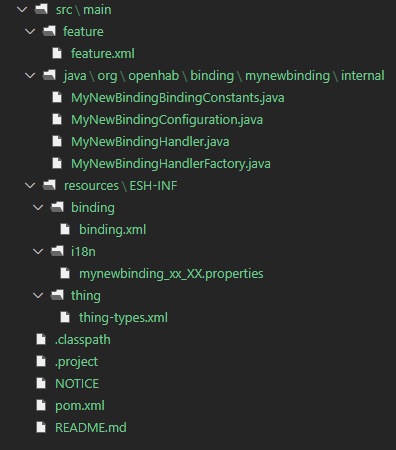
\includegraphics[width=0.5\textwidth]{\figdir/own_binding_skeletton.PNG}
	\caption{Skelett für Binding \label{fig:own_binding_skeleton}}
}

Die Binding-Vorlage gibt u.a. vor, dass im XML-Format beschrieben werden muss zu welchem Gerät das Binding gehört und welche Things inklusive Channels erzeugt werden. In Java werden benötigte Binding-Handler und Konfigurationen geschrieben. Codebeispiel \ref{lst:binding-coding} kann entnommen werden, wie intensiv die Unterstützung durch die Binding-Vorlage ist. So wird nicht nur mit einem Beispiel gezeigt, wie auf Informationen, welche durch einen Channel übertragen werden reagiert werden kann, sondern auch auf Besonderheiten hingewiesen und was in welcher Funktion zu entwickeln ist.


\begin{lstlisting}[language=java,firstnumber=1,caption=Handler.java Ausschnitt,label=lst:binding-coding]
xxxBindingHandler.java
...
@Override
public void handleCommand(ChannelUID channelUID, Command command) {
if (CHANNEL_1.equals(channelUID.getId())) {
if (command instanceof RefreshType) {
// TODO: handle data refresh
}

// TODO: handle command

// Note: if communication with thing fails for some reason,
// indicate that by setting the status with detail information:
// updateStatus(ThingStatus.OFFLINE, ThingStatusDetail.COMMUNICATION_ERROR,
// "Could not control device at IP address x.x.x.x");
}
}

@Override
public void initialize() {
// logger.debug("Start initializing!");
config = getConfigAs(MyNewBindingConfiguration.class);

// TODO: Initialize the handler.
// The framework requires you to return from this method quickly. Also, before leaving this method a thing
// status from one of ONLINE, OFFLINE or UNKNOWN must be set. This might already be the real thing status in
...
\end{lstlisting}


\section{Verwendung von openHAB}
\label{s:usage-open-hab}


\subsection{Beispiel Aufbau eines openHAB Smart-Homes}
	Um mit openHAB Erfahrungen zu sammeln wurde für das Projekt ein eigenes Smart-Home System erstellt. Dabei wurde darauf geachtet ein praktisches System zu erstellen, dass die üblichen Anforderungen an ein Smart-Home erfüllt und zudem eine gute Übersicht über die Grenzen und Möglichkeiten von openHAB geben kann.

	\subsubsection{Hardware für openHAB}
		Für das System wurde ein Raspberry pi der vierten Generation mit 2gb Arbeitsspeicher gewählt. Der Raspberry ist mit Wlan und Bluetooth ausgestattet. Darauf wird openHABian installiert. Dies ist ein an openHAB angepasstes Linux Buster Betriebssystem. Mit openHABian kommt die neuste Version von openHAB und nützliche Systemlibraries und Einstellungen, um besser mit openHAB arbeiten zu können. Damit ist der Raspberry pi bereits fertig eingerichtet und openHAB startet automatisch beim Systemstart. Die Weboberfläche wird im Netzwerk unter https://openHAB:8080 bereitgestellt. Dort können die meisten Einstellungen vorgenommen werden, um Geräte und Systeme einzubinden und eine Benutzeroberfläche zum Steuern des Systems zu erstellen. Über SSH ist ein Zugriff direkt auf den Raspberry pi möglich. Ein SSH Zugriff ist für verschiedene Anpassungen nötig, die den Raspberry selbst betreffen oder nicht über die Bereitgestellte Weboberfläche umsetzbar sind.
		Damit das System später leicht bedienbar ist, wird ein 7 Zoll Touch-Monitor verwendet um ein HAB Panel anzuzeigen. Dank Touch-Funktionalität funktioniert er als Steuersystem und das System kann jederzeit bedient werden.
		
	\subsubsection{Eingebundene Geräte}
		In openHAB lassen sich eine Vielzahl an Geräten und Services einbinden. Für unsere Arbeit wählen wir exemplarisch verschiedene Geräte aus, die in einem üblichen Wohnzimmer nützlich sind.
		\begin{itemize}
			\item Hue Bridge
			\item  hue LED
			\item Osram Lightify LED
			\item LG Smart TV
		\end{itemize}
		Beide Lampen arbeiten mit dem Zigbee Protokoll welches eine eigene Frequenz verwendet und somit leicht bis zu 50 Geräte verwalten kann. Dadurch kommuniziert unser System immer nur mit der Hue Bridge, wenn die Lampen angesprochen werden sollen. Dies passiert allerdings im Hintergrund, in der openHAB Weboberfläche stellt uns die hue Bridge jede Lampe als eigenes Item dar.
		
		Bei beiden Lampen lässt sich Helligkeit und Farbtemperatur anpassen. Der Fernseher lässt sich an und ausschalten und die Lautstärke und das Programm verändern.
		
		\subsubsection{Eingebundene Services}
		Das System soll die Möglichkeit Musik zu steuern integrieren und aktuelle Wetterdaten anzeigen. Dazu wählen wir Spotify als Musikanbieter und openWeatherMap um die Wetterdaten abzurufen. Beide Dienste sind in einer kostenlosen Version nutzbar und daher als Beispiel sinnvoll.
		
		Spotify ermöglicht es über die Developer Webseite von Spotify eine Webanwendung zu registrieren. Damit kann unser System sich autorisieren einen Spotify Account zu steuern. Das System schickt dabei Befehle an die Server von Spotify, welche wiederum die Befehle an den aktuellen Spotify Client weiterleiten. Es muss also nicht direkt Spotify auf dem Raspberry installiert werden. Das steigert die Performance und ist in der Handhabung angenehmer. Das System soll das aktuelle Lied anzeigen und es ermöglichen Lautstärke zu verändern, den Track zu wechseln und die Wiedergabe zu starten und stoppen.
		
		Um die Wetterdaten abzurufen ist ein Account bei openWeatherMap nötig. Für das System wird die kostenlose Basisversion gewählt. Mit dem Account ist ein API Key verknüpft, um das System zu authentifizieren. Mit der Basisversion können wir die aktuellen Wetterdaten verschiedener Standorte abrufen werden.
		
		\subsubsection{Integration der Geräte und Services}
		Die Integration der Geräte erfolgt über die Paper UI des Webfrontend, dass das openHAB System bereitstellt. 
		
		Für die Integration der Lampen müssen diese zuerst über die hue App mit der hue Bridge verbunden werden. Danach wird das hue Binding installiert. Die IP Adresse der Bridge  muss konfiguriert werden und das System erkennt dann die Bridge automatisch. Die Bridge kann jetzt als Thing in das System aufgenommen werden. Dadurch wird auch automatisch die Lampen als Things erstellt. Für alle drei Lampen werden je zwei Items angelegt, um Helligkeit und Lampenfarbe steuern zu können. Diese Items erlauben es, auch den aktuellen Wert auszulesen. Da die Osram Lampe das Lightify protokoll nutzt, welches die hue Bridge ebenfalls unterstützt, funktioniert die Einrichtung dort identisch.
		
		Der LG Smart TV wird mit dem LG WebOS Binding integriert. Nach Installation wird der Fernseher von alleine erkannt wenn er im selben Netzwerk ist. Es können dann Items erzeugt werden, um den Fernseher an- und auszuschalten und die Lautstärke zu regeln.
		
		Spotify wird über das Spotify Binding integriert. Es muss ClientId und Secret Key hinterlegt werden, welche in der Spotify Developer Console angelegt wurden. Das Binding erstellt ein Spotify Player Bridge Thing mit welchem nun ein Spotify Account gesteuert werden kann. Es werden Items erzeugt, um den Songtitel auslesen zu können und zwei weitere um die Lautstärke und den Player zu kontrollieren. Der Spotify Musik Player wird dabei als Media Controler Item erzeugt und kann die Wiedergabe stoppen oder starten und Lieder wechseln.
		
		Um Wetterdaten abrufen zu können, wird das Weather Binding benötigt. Für dieses Binding ist eine manuelle Einrichtung auf dem Raspberry nötig. Per SSH muss die services/weather.cfg angepasst werden.
		
		\begin{lstlisting}[language=java,firstnumber=1,caption=services/weather.cfg,label=code-weatherlocation]
apikey.openWeatherMap=sdf7g69fdgdfg679dfg69sdgkj
location.home.provider=openWeatherMap
location.home.language=de
location.home.updateInterval=10
location.home.latitude=47.8011
location.home.longitude=13.0448
		\end{lstlisting}
		
		Wie in Abbildung \ref{fig:code-weatherlocation} zu sehen ist, wurde der API Key für openWeatherMap hinterlegt und eine Locations names "`home"' angelegt. Für diese wurde auch die Latitude und Longitude hinterlegt, sodass unsere Wetterdaten für diesen Ort abgerufen werden können. Der updateInterval 10 gibt an, dass die Wetterdaten alle 10 Minuten erneut geladen werden.
		Nach diesen Einstellungen können Items erzeugt werden.
		
				\begin{lstlisting}[language=bash, escapeinside={(*}{*)} ,firstnumber=1,caption=items/weather.items,label=code-weatheritems]
Number   Temperature   "Temperature [%.2f (*°*)C]"
{weather="locationId=home, type=temperature, property=current"}
Number   Precip_Probability   "Precip probability [%d %%]"
{weather="locationId=home, type=precipitation, property=probability"}
Number   Wind_Speed           "Windspeed [%.2f km/h]"
{weather="locationId=home, type=wind, property=speed"}
		\end{lstlisting}
		
		Das Item File der Wetter Items aus Abbildung \ref{fig:code-weatheritems} erzeugt drei Items welche die Temperatur, die Niederschlagswahrscheinlichkeit und die Windgeschwindigkeit beinhalten.
		Es wird bei den Items die weatherId "`home"' verwendet. Dadurch benutzt das Binding bei der Abfrage der Daten die zuvor erzeugten Ortsdaten.
		
		\subsubsection{Erstellung des HAB Panels}
		Ein HAB Panel kann auf der Web UI aus verschiedenen Widgets und Items zusammengestellt werden. Dabei werden einzelne Widgets auf Dashboards angeordnet und dann mit verschiedenen Items verknüpft. Es kann z.B. ein Slider angelegt werden, welche die Helligkeit der Lampen regelt. Einzelne Items können dabei beliebig oft verwendet werden. So kann es neben dem Slider z.B. auch noch einen Button geben, der die Helligkeit zwischen 100 Prozent oder 0 Prozent wechselt. Damit kann die Lampe ein und ausgeschaltet werden.
		
		Für das Panel des Smart Home Systems werden Standardkomponenten, Widgets aus dem Community Store und auf selbst erstellte Widgets zurück. Eigene Widgets können als Angular Widget erstellt werden.
		
	\begin{minipage}{\textwidth}
		\centering
		\captionsetup{type=figure}
		\includegraphics[width=1\textwidth]{\figdir/openHABPanel.png}
		\caption{Erstelltes openHAB Panel \label{fig:activity-diagram}}
	\end{minipage}
		
		In Abbildung /ref{} sehen wir das erstellte Panel. Darauf ist zuerst der Namen des Dashboardes "`Home"' und darunter die aktuelle Uhrzeit dargestellt. Letzteres ist ein Standardwidget von openHAB.
		Darunter ist ein Label, welches den aktuellen Songtitel von Spotify anzeigt und ein vom Community Store eingebundener Music Controller, welcher Track und Lautstärke von Spotify steuern kann.

		Ganz unten befindet sich ein selbst geschriebenes Widget, welches die Wetterdaten anzeigt.

		In der rechten unteren Ecke befinden sich zwei Buttons, um den Raspberry neuzustarten oder auszuschalten. Diese können über das Exec Binding Befehle in der Kommandozeile ausführen.
		
		Unten in der Mitte befindet sich die Steuerung des Fernsehers. Der Linke Button schaltet ihn an und aus, der Slide regelt die Lautstärke.
		
		Alle restlichen Widgets steuern die Lampen. Das große Widget kann alle Lampen im Zimmer an und ausschalten. Die kleinen Widget präsentieren die einzelnen Lampen. Über die Slider lässt sich die Helligkeit und Weißfarbe aller Lampen einstellen.
		
		\subsubsection{Kontrollstation einrichten}
		Um das System bequem steuern zu können, wird eine Kontrollstation aus dem Raspberry pi selbst und einem 7 Zoll Bildschirm errichtet. Es wird dafür ein Bildschirm gewählt, auf welchem sich der Raspberry befestigen lässt und direkt vom Raspberry Strom bezieht.
		Die Kontrollstation wird dann das erstellte HAB Panel anzeigen und so Zugriff auf das System ermöglichen.

		Um auf dem Raspberry pi eine Benutzeroberfläche anzeigen zu können, PIXEL installiert werden. Dabei wird der Browser Chromium mit ausgeliefert. Es müssen verschiedene Einstellungen vorgenommen werden, damit der Raspberry pi ohne Login startet und direkt Chromium öffnet. Gleichzeitig soll der Mauszeiger ausgeblendet werden und das Panel im Vollbildmodus anzeigen. Alle Einstellungen können nicht mit openHAB erledigt werden. Per SSH müssen diese direkt auf dem Raspberry pi vorgenommen werden.

		\subsubsection{Externer Zugriff}
		Eine häufige Anforderung an Smart Home Systeme ist auch extern auf das System zugreifen zu können. So kann auch von unterwegs der Zustand der Geräte kontrolliert werden und diese auch gesteuert werden. Für openHAB gibt es die myopenHAB Cloud. Für diese muss das open Hab Cloud Connector Addon installiert werden. Dieses erzeugt auf dem Pi ein Secret File mit einem Secret Key. Registriert man einen Account bei myopenHAB, muss dieser Secret-Key und ein von openHAB erzeugte UUID hinterlegt werden. Danach ermöglicht das Addon eine Verbindung nach außen zur myopenHAB Cloud.
		In myopenHAB können erstellte Panels angezeigt werden mit denen das Gerät wie gewohnt gesteuert werden kann. Das ganze System kann jetzt auch extern bearbeitet werden. MyopenHAB gibt dabei die Möglichkeit auf das System zuzugreifen als wäre man im selben Netzwerk.
		Es gibt für die myopenHAB Cloud auch Smartphone Apps für Android und iOS. Nach der Anmeldung mit dem myopenHAB Account ist ein sichere Zugriff auf das System auch von unterwegs möglich. Dabei kann auf Panels zugriffen werden und Items direkt gesteuert werden. Allerdings sollte das Panel auf die Größe des Smartphone Bildschirms angepasst werden, oder eigene Panels für Mobile Geräte erstellt werden.
		
		
		\subsection{Verteilungsarchitektur des Smart Home Systems}
		
\begin{minipage}{\textwidth}
	\centering
	\captionsetup{type=figure}
	\includegraphics[width=1\textwidth]{\figdir/VerteilungsarchitekturopenHAB.png}
	\caption{Verteilungsarchitektur des Smart Home Systems \label{fig:activity-diagram}}
\end{minipage}

	Abbildung \ref stellt die Verteilungsarchitektur des erstellten Smart Home Systems dar. In der Darstellung sind Hardwarekomponenten durch einfache Rechtecke dargestellt und Softwarekomponenten durch Rechtecke mit zwei vertikalen Linien. Die Verteilungsarchitektur zeigt die verschiedenen Geräte und Services und wie sie mit openHAB verbunden sind. Dabei sind alle Services und Geräte über Bindings verbunden. Der Touch Monitor ist direkt über HDMI mit dem Raspberry pi verbunden und zeigt das HAB Panel an, welches von der Weboberfläche des open HAB Systems bereitgestellt wird. Das hue Binding spricht die hue Bridge an, welche dann die Lampen steuert.
	
\subsection{Integration der Big Player}
Amazon Alexa und Google Home sind die bekanntesten Voice Services laut Google Trends. \cite{GOOGLET01:AG} Damit ist es möglich über verbale Kommandos bestimmte Funktionalitäten anzusteuern. Beispielsweise das abspielen eines Radiosenders oder das An- und Ausschalten einer Lampe.\\
Sowohl der Google Home Assistent als auch Amazons Alexa sind in das Heimautomatisierungstool openHAB integrierbar.In den folgenden zwei Unterkapiteln wird dies genauer erläutert.\cite{openHAB02:OH}

\subsubsection{Amazon Alexa}
In openHAB kann ein zertifizierter Amazon Alexa Smart Home Skill verwendet werden. Damit ist es möglich eine ganzes Smart Home durch verbale Kommandos zu verwenden. Es können dadurch Lichter, Schlösser, Thermostate, Sensoren und viele weitere Geräte angesteuert werden. Dies ist möglich durch Alexa oder den Echo Dot.\cite{ALEXA01:AL}\cite{ALEXA02:AL}
Um die Geräte von Amazon als Eingabe nutzen zu können, wird zusätzlich die Verbindung zur myopenHAB Cloud benötigt, da diese die Verarbeitung der Kommandos an Amazon weiterleitet.\\
\\
Seit der Version 2.5 nutzt der Alexa Skill von openHAB die neuste Smart Home Skill API V3. Dadurch können nun viele Smart Home Geräte deutlich vielseitiger und präziser angesprochen werden. Außerdem unterstützt der Skill nun alle 15 Sprachen, in denen Alexa verwendet werden kann. Weiterhin ist Abwärtskompatibilität zu früheren Versionen gewährleistet.\cite{openHAB02:OH}

\subsubsection{Google Home}

Prinzipiell sind mithilfe von Google Home fast alle Optionen gegeben, die auch durch Amazons Alexa existieren. Somit können ebenfalls verschiedenste Geräte angesteuert werden. Für die Verwendung wird, wie beim Amazon Skill, eine Verbindung mit der myopenHAB Cloud benötigt.\\
\\
Beim letzten Update von openHAB wurde die Anwendung von Google Home ebenfalls verbessert. Dabei ist sowohl die Codequalität als auch die Sicherheit der Integration gesteigert worden. Weiterhin ist es durch die neuste Version möglich, deutlich mehr Features der Google Smart Home API zu nutzen. Dabei wurden sowohl neue Funktionen als auch der Support für alle Sprachen eingebaut.\cite{openHAB02:OH}\cite{GOOGLEH01:GH}

\section{Datenintegrität und Sicherheit}

Dieses Kapitel bietet einen Überblick über die Sicherheit im Internet-of-Things-Bereich (IoT).  Anschließend wird auf die Sicherheit in openHAB selbst und dafür verwendbare Erweiterungen eingegangen. Dies beinhaltet außerdem mögliche Sicherheitslücken und dazugehörige Gegenmaßnahmen.\\
\\
Open Web Appliation Security Projekt (OWASP), eine Community, die frei erhältliche Artikel zur Sicherheit im Internet bereitstellt, veröffentlichte 2019 eine Liste der Top Sicherheitsbedrohungen aus dem Jahr 2018 im Iot-Bereich.\cite{OWASP01:IOT} Das dabei größte Sicherheitsrisiko besteht bei schwachen, einfach erratbaren oder hart-kodierten Passwörtern. Dies wird von OWASP beschrieben mit "`Use of easily bruteforced, publicly available, or unchangeable credentials, including backdoors in firmware or client software that grants unauthorized access to deployed systems"'.\cite{OWASP01:IOT} Auf Platz 2 und 3 befinden sich unsichere Netzwerk Services und Ecosystem Interfaces. Damit sind indirekte Zugriffsmöglichkeiten durch ungesicherte Services gemeint, die entweder von innerhalb oder außerhalb des IoT-Netzwerks erreichbar sind. Sobald ein Angreifer diesen Service "`übernommen"' hat, kann dieser problemlos Zugriff erlangen, wenn keine Sicherheitsvorkehrungen diesbezüglich getroffen wurden.\\
\\
openHAB in der Version 2.4 wird in der Masterarbeit von Jesús Antonio Soto Velázquez über "`Securing openHAB Smart Home through User Authentication and Authorization"', auf Sicherheit geprüft.\cite{MA01:OPH} Dabei untersucht der Autor mithilfe von Wireshark, wie openHAB kommuniziert und kommt zu dem Resultat, dass es drei verschiedene Kommunikationsszenarien gibt, die sicherheitstechnische Relevanz haben. Alle drei Szenarien nutzen Bindings als Mittel der Kommunikation. Diese sind:
\begin{itemize}
	\item intern: Thing - openHAB
	\item extern mit logischem Thing: openHAB-Remote Web Service
	\item extern mit physikalischem Thing: openHAB-Remote Web Service Thing
\end{itemize}	
Interne Kommunikation zwischen Thing und openHAB Instanz findet typischerweise über WLAN statt, welches mithilfe von AES verschlüsselt ist. Um in das System einzudringen, müsste ein Angreifer entweder AES entschlüsseln können oder das Passwort anderweitig herausfinden. AES gilt als nicht entschlüsselbar in einer annehmbaren Zeit. Daraus lässt sich schließen, dass die interne Kommunikation von openHAB und Things nur so sicher ist, wie das ganze WLAN-Netzwerk selbst.\\
Bei den zwei externen Punkten sind laut 
Jesús Antonio Soto Velázquez nur Lauschangriffe möglich. Normalerweise sollten externe Thing's mit openHAB und Cloud ausschließlich über das Hyper Transfer Protocol Secure (HTTPS) miteinander kommunizieren. Dabei hängt es von der jeweiligen Implementierung von Binding und Aufrufen für die Datenübermittlung ab, ob HTTPS oder dessen unverschlüsselte Form HTTP eingesetzt wird. Weiterhin weißt der Autor darauf hin, dass sobald ein Binding Daten unverschlüsselt über das Internet verschickt, andere Bindings davon nicht betroffen sind. Diese gelten weiterhin als sicher, solange der Angreifer nicht über andere Wege in das System eingedrungen ist.\\
\\
Trotz der Untersuchung der nicht ganz aktuellen Version 2.4, ist der Inhalt dieser Masterarbeit aktuell, denn mit der Version 2.5 wurden kaum Updates bezüglich Sicherheit integriert.\cite{openHAB02:OH} Folglich wird auf die sowohl internen als auch externen Sicherheits-Features von openHAB detaillierter eingegangen.

\subsection{Interne vorhandene Funktionalitäten}
openHAB bietet bereits ein paar Sicherheitsvorkehrungen "`out-of-box"' an. Grundsätzlich kann die openHAB Instanz nur über Secure Shell (SSH) oder HTTP/HTTPS erreicht werden. Bei der Kommunikation über SSH wird, wie bereits erwähnt, das als sicher geltende AES verwendet. HTTPS hingegen nutzt Zertifikate und wird zur Herstellung von Integrität und Vertraulichkeit der Kommunikation zwischen Client und Server im Internet verwendet. Es gilt ebenfalls als sicher.\\
Beim ersten Aufsetzen von openHAB wird ein selbst-signiertes SSL-Zertifikat (256-bit ECC) erstellt und im Jetty (Webservice) Keystore gespeichert. Dadurch kann sichergestellt werden, dass jede openHAB Instanz eindeutig ist. Ein potenzieller Angreifer kann demzufolge keinen Evil-Twin (Böser Zwilling) aufbauen und ein openHAB System nachahmen.\\
\\
Die Abbildung \ref{fig:verteilungs-architektur} zeigt eine Verteilungsarchitektur mit den verwendeten Protokolle einzelner openHAB-Komponenten aus Kapitel \ref{s:usage-open-hab}.\\
\begin{minipage}{\textwidth}
	\centering
	\captionsetup{type=figure}
	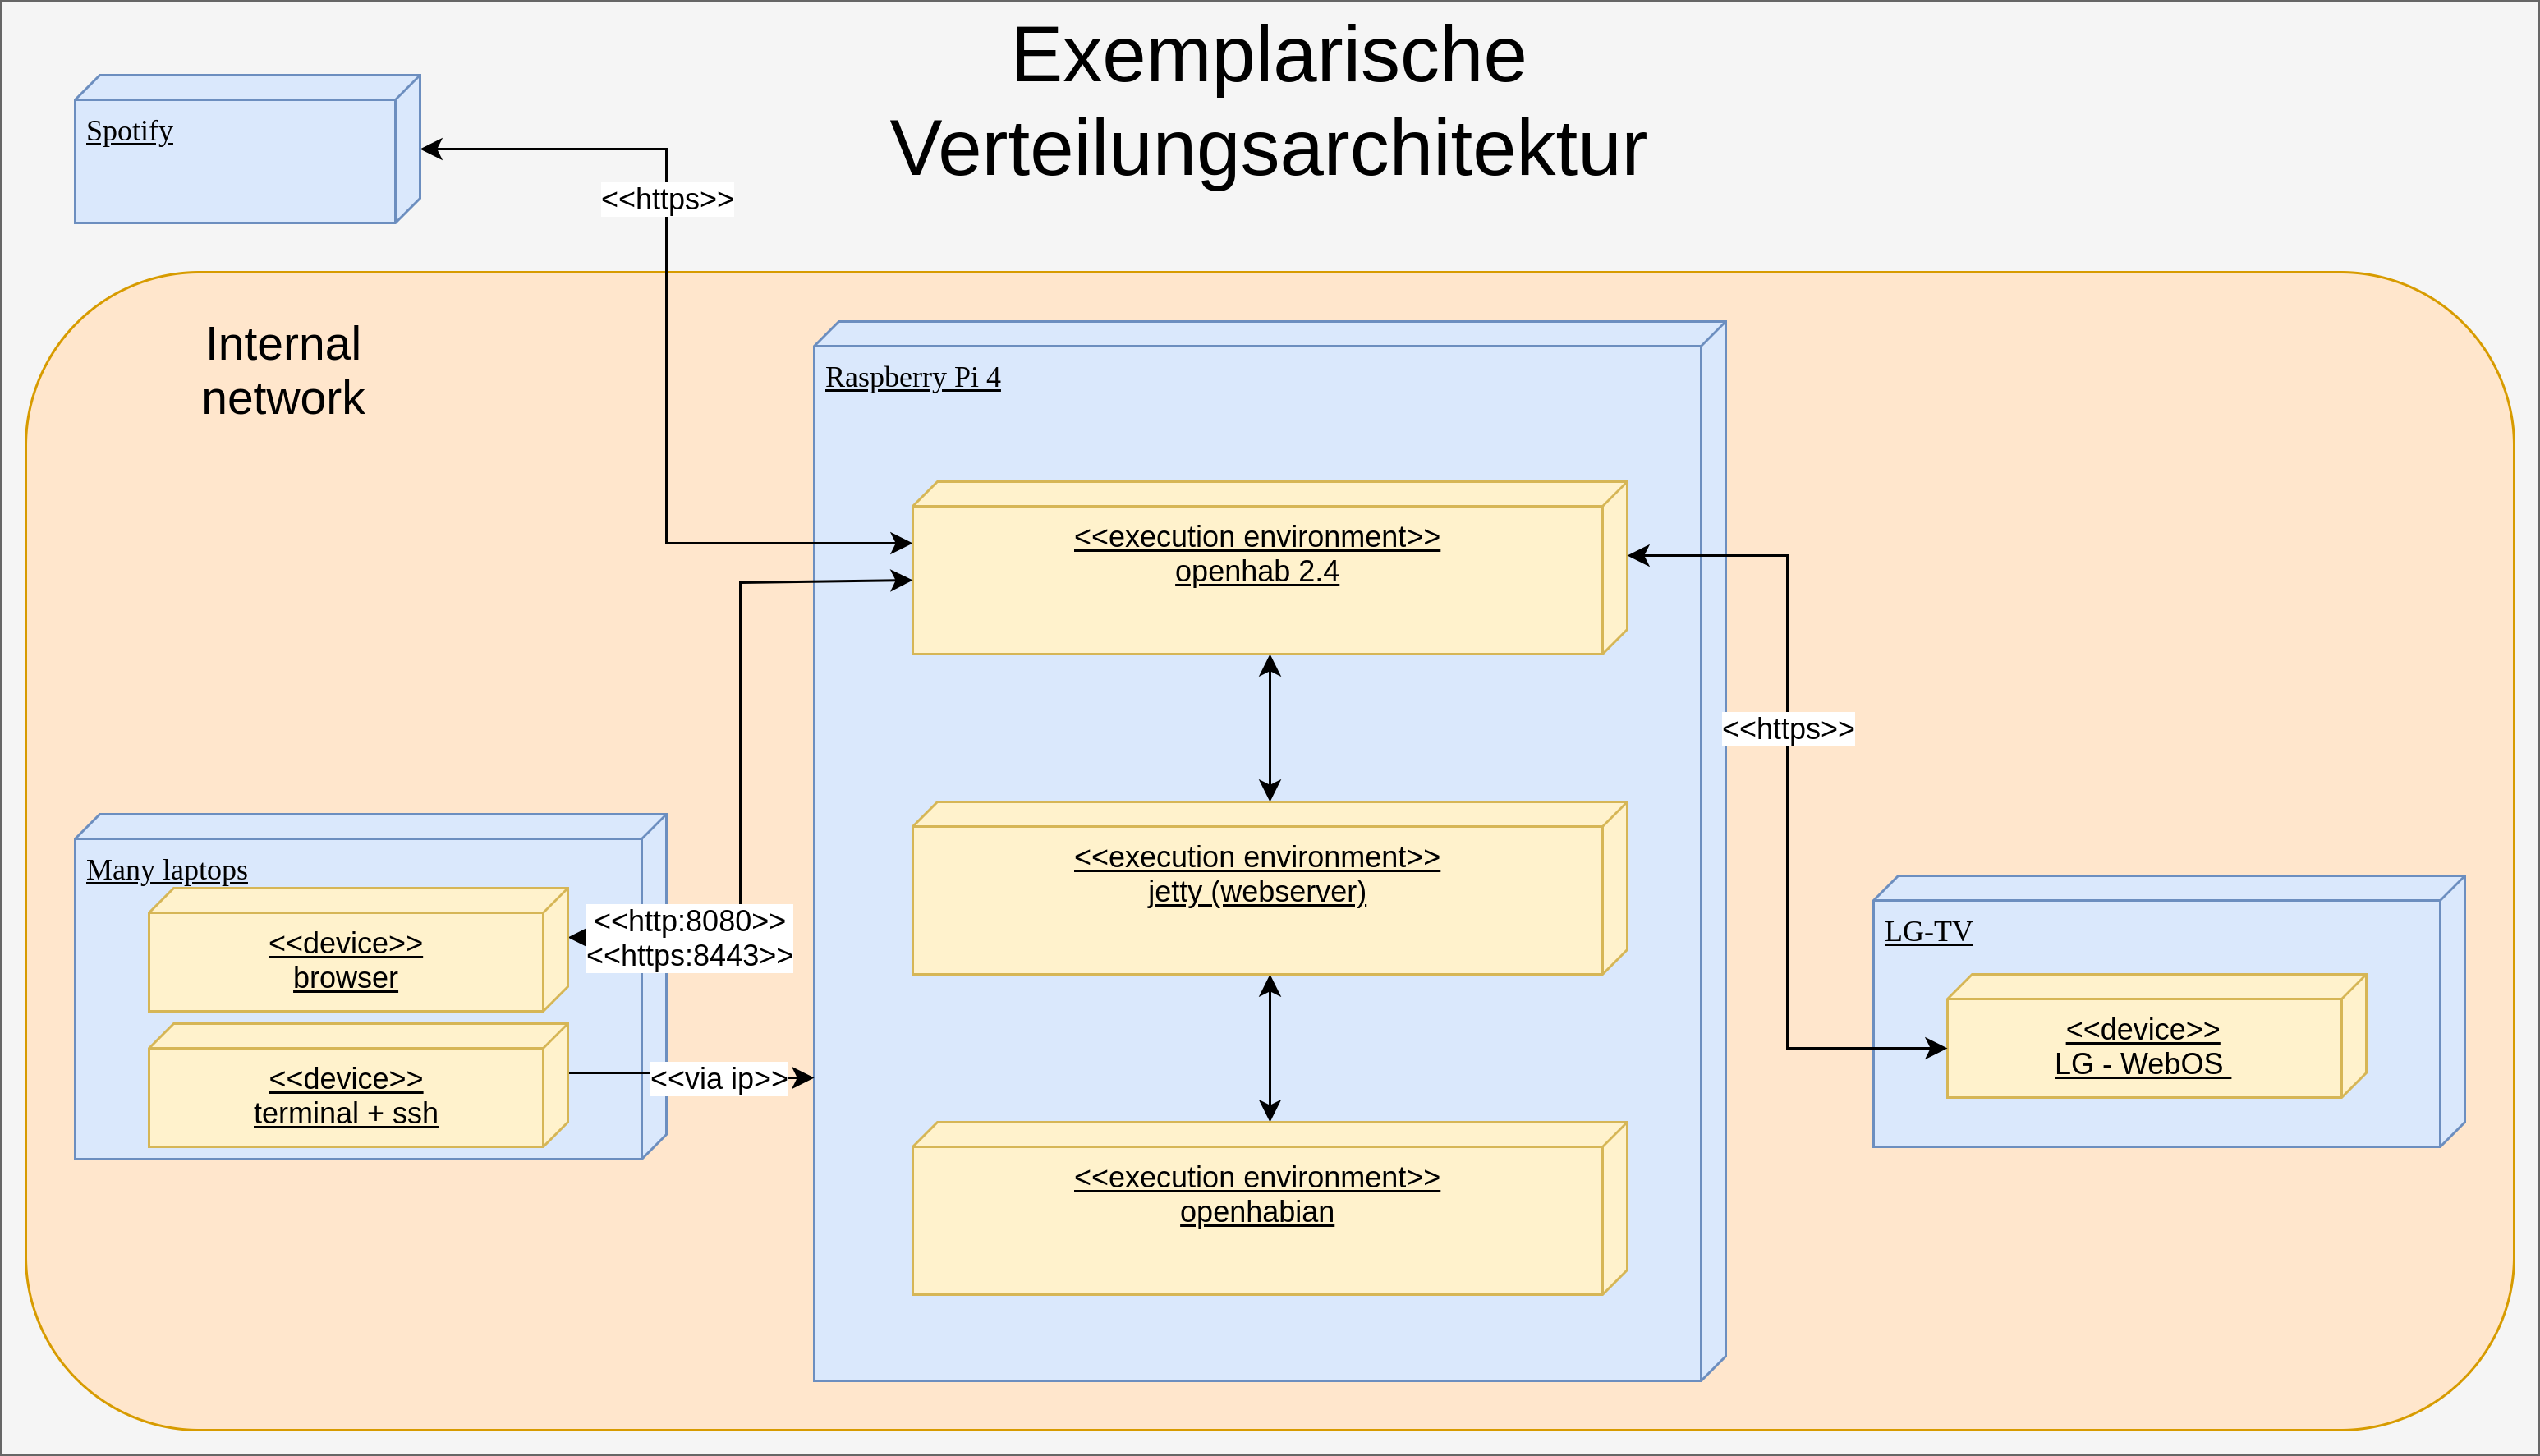
\includegraphics[width=1\textwidth]{\figdir/verteilungsarchitektur.png}
	\caption{Übersicht einer exemplarischen Anwendung von openHAB \label{fig:verteilungs-architektur}}
\end{minipage}
\\
\\
Die darin zu sehenden Komponenten sind durch einen blauen Hintergrund markiert. Die jeweils darauf laufende Software ist durch die Farbe Gelb dargestellt. Alles bis auf Spotify ist im internen Netzwerk abgebildet (orange eingegrenzten Bereich).\\
Die jeweiligen Komponenten kommunizieren mit der zentralen openHAB Instanz, welche auf einem Raspberry Pi gehostet wird. Dabei sind die verwendeten Protokolle für die Informationsübertragung auf den gerichteten Pfeilen zu sehen.

\subsection{Externe Erweiterungsmöglichkeiten}
Ein weiterer Weg der Benutzung einer openHAB-Instanz wäre dies von außerhalb des Heimnetzwerks über beispielsweise das Smartphone zu erreichen. Hierfür werden die "`Best Practices"' in der openHAB Dokumentation erläutert.\\
Dabei wird eine VPN Verbindung in das Heimnetzwerk als sicherster Weg bewertet. Den openHAB Cloud Service zu nutzen, ist eine weitere Möglichkeit. Dabei wird ebenfalls eine Tunnelverbindung aufbaut, wodurch openHAB durch die Cloud angesteuert wird.\\
Schlussendlich kann openHAB hinter einem Reverse Proxy betrieben werden. Dieser leitet Client-Anfragen weiter an den gewünschten Server. Damit ist es möglich über den Proxy auf die im Heimnetzwerk eingesetzt openHAB-Instanz über eine bestimmte Domain zuzugreifen.\\
\\
Weiterhin warnt openHAB auf ihrer Website davor, Ports an der Firewall für openHAB zu öffnen. Es wird ausdrücklich gesagt, dass dies in keinem Fall benötigt wird.\cite{openHAB03:OH}

\section{Fazit}
\subsection{Zusammenfassung}
Diese Arbeit analysiert das open-source Heimautomatisierungstool openHAB auf Markttauglichkeit und Benutzbarkeit. Zu Beginn wird dafür erklärt, was openHAB ist und wofür es verwendet werden soll. Anschließend folgt eine Bewertung des Projektes mithilfe von Open Hub und einer Facharbeit. Das daraus resultierende Ergebnis besagt, dass openHAB ein gutes Heimautomatisierungstool ist und auch im Vergleich zu seinesgleichen auf dem Markt etabliert ist.\\
Weiterhin werden die technischen Grundlagen, Programmier-Schnittstellen und mehrere Anwendungsbeispiele in den darauffolgenden Kapiteln erläutert.\\
Abschließend geht diese Arbeit auf Datenintegrität und Sicherheit ein.

\subsection{Schlussfolgerung}
Heimautomatisierungstools werden immer notwendiger, um mit dem wachsenden Markt im Bereich Iot mithalten zu können.\cite{STATISTA01:IOT} Das bekannte open-source Tool openHAB bietet die fundamentalen Funktionalitäten für Heimautomatisierung. Dies bekräftigt auch das Ergebnis dieser Arbeit. Dabei wurde festgestellt, dass openHAB aktiv von einer wachsenden Community weiterentwickelt wird und sowohl privat als auch kommerziell eingesetzt werden kann, da das Projekt unter einer EPL-2.0 Lizenz steht.\\
Die Komponenten aus denen openHAB besteht, bzw. die Teile, welche einem Benutzer zur Verfügung stehen, sind klar strukturiert und besitzen eine Abstraktionsstufe, die gut verständlich ist. Auch wenn die Namensgebung der Items nicht optimal ist, wird ersichtlich wie der Zusammenhang zwischen Bindings, Things, Channels und Items ist. openHAB bietet durch die Add-On Architektur einige Möglichkeiten der Erweiterung. Dies wird im Falle von Bindings noch durch die bereitgestellten Skripte vereinfacht, was dazu führt, dass openHAB relativ einfach um neue Geräte erweitert werden kann.\\
Weiterhin wurde festgestellt, dass openHAB selbst sichere Verbindungen beim Austausch von Informationen über Geräte nutzt. Dabei wird für Zugriffe von innerhalb und außerhalb des Netzwerks auf die Technologien HTTPS und SSH gesetzt. Das einzige aktuelle Sicherheitsproblem ist, dass ältere integrierbare Bindings, welche meist durch Dritte geschrieben wurde, HTTP verwenden. Da sowohl HTTPS als auch SSH als sicher gelten, sind nur über die unsicheren HTTP Verbindungen Lauschangriffe möglich, sofern sich keine anderen Lücken im System befinden.
\\
Die Autoren dieser Arbeit bewerten openHAB als gut gelungenes Heimautomatisierungstool. Nach einer gewissen Einarbeitungszeit ist das Zusammenbauen eines Smart Homes damit unkompliziert umsetzbar. Es erlaubt die Einbindung fast aller Geräten aus dem Iot-Bereich, erfordert jedoch an manchen Stellen Kenntnisse in der Softwareentwicklung.


\subsection{Ausblick}
Mit dem Release 2.5 Ende 2019 ist offiziell die Entwicklung an Version 3.0 gestartet. Version 2.5 wird allerdings weiter gepflegt werden. Für die Version 3 sind einige Breaking Changes geplant. So soll vor allem die verschiedenen UI's (Paper UI, Basic UI, und mehr) zusammengeführt werden und das erstellen von Rules wird überarbeitet.\cite{openHAB02:OH} Da das Projekt Open Source von der Community entwickelt wird kann sich an diesem Plan etwas ändern. Der Ausblick lässt aber vermuten, dass bereits jetzt ein gute Schwerpunkt gelegt wurde und openHAB mit der nächsten Version einen weiteren Schritt nach vorne machen wird. Es steht derzeit noch kein Release Datum fest. Da wichtige Releases in der Vergangenheit oft am Ende des Jahres zur Weihnachtszeit veröffentlicht wurden, liegt es nahe, dass frühestens Ende 2020 damit zu rechnen ist.

%%% Local Variables: 
%%% mode: latex
%%% TeX-master: "thesis.tex"
%%% End: 
